
% Modelo de slides para projetos de disciplinas do Abel
\documentclass[10pt]{beamer}

\usetheme[progressbar=frametitle]{metropolis}
\usepackage{appendixnumberbeamer}
\usepackage[numbers,sort&compress]{natbib}
\bibliographystyle{plainnat}

\usepackage{booktabs}
\usepackage{epstopdf,subfigure}
\usepackage[scale=2]{ccicons}

\usepackage{xspace}
\newcommand{\themename}{\textbf{\textsc{metropolis}}\xspace}

\title{IPSW - Modelling Change of Website Archives}
\subtitle{Group 4}
\date{\today}
%\date{}
\author{Ian Milligan, Ian Roper, Caoimhe Rooney, \\Nathan Taback, Jessica Williams, Nich Worby}
%\institute{UFPR - Disciplina - Semestre}
% \titlegraphic{\hfill\includegraphics[height=1.5cm]{logo.pdf}}

\begin{document}

\maketitle

%%\begin{frame}{Table of contents}
 % \setbeamertemplate{section in toc}[sections numbered]
 % \tableofcontents[hideallsubsections]
%\end{frame}

\section{The Problem}

\begin{frame}{The Problem}

\large

\begin{itemize}
\item Decades of web archives with lots of vital historic information 
\item Gets overridden from history when the website is updated
\item Ever increasing amount of data
\item Scale overwhelms the search for the meaningful information
\end{itemize}

\pause

\vspace{5mm}

Can we
\begin{itemize}
\item find out when large changes have occurred?
\item predict when a big change is going to occur?
\end{itemize}

\end{frame}

\begin{frame}{Aims for this week}

\Large

\begin{itemize}
\itemsep1.0em
\item Find and explore ways to quantify change in a website
\item Compare these quantifications
\item See if we can identify big changes in an organisation from our research
\end{itemize}

\end{frame}

\begin{frame}{Big events in the NDP}

\begin{itemize}
\item 28 November 2005: election called.
\item 23 January 2006: federal election.
\item 14 October 2008: federal election.
\item 2 May 2011: federal election.
\item July 2011: NDP leader announces leave of absence; replaced by interim.
\item 22 August 2011: NDP leader dies.
\item 24 March 2012: New NDP leader selected.
\item 19 October 2015: federal election.
\item 10 April 2016: NDP leader loses vote of confidence.
\item 1 October 2017: New NDP leader selected.
\end{itemize}

\end{frame}

\begin{frame}{Attempted Approaches}
\Large
\begin{itemize}
\itemsep1.0em
\item How much words on the domain change
\item How the links out of the domain change
\item How the way the domain looks changes
\item How the structure of the websites within the domain change
\end{itemize}
\end{frame}

\begin{frame}{Four Metrics for Text}
%\vspace{-4mm}
%\LARGE Four metrics:\\
%\vspace{2mm}
\begin{minipage}{0.6\textwidth}
\begin{itemize}
\large\item Byte-wise comparison:
\begin{itemize}
\item If any change in characters has occurred, = 1
\item If text is \textit{exactly} the same, = 0
\end{itemize}
\item TF$\cdot$IDF \\
\begin{itemize}
\item Calculates cosine distance between two different vectors of characters $\boldsymbol{p}$ and $\boldsymbol{p}'$
\end{itemize}
\item Word distance
\begin{itemize}
\item How many words have changed
\end{itemize}
\item Edit distance
\begin{itemize}
\item ``Edit distance'' $\delta$ is the amount of insertion/deletion/substitution needed to turn one sequence into the other
\end{itemize}
\end{itemize}
\end{minipage}
\begin{minipage}{0.38\textwidth}
\Large
\vspace{10mm}
\begin{equation*}
1-\frac{\boldsymbol{p}\cdot \boldsymbol{p}'}{||\boldsymbol{p}||_2||\boldsymbol{p}'||_2}
\end{equation*}
\vspace{5mm}
\begin{equation*}
1-\frac{2|common \text{ } words|}{m+n}
\end{equation*}
\vspace{1mm}
\begin{equation*}
\frac{\delta}{m + n}
\end{equation*}
\end{minipage}
\end{frame}

\begin{frame}{External Links}

\Large
\begin{itemize}
\item Justification
\begin{itemize}
\large\item Links to other websites are important to the website designer
\item If these change, the topic of the website has most likely changed as well
\end{itemize}
\item Method
\begin{itemize}
\item Compare vector of links on homepage at $t_i$ and $t_{i+1}$ as $\textbf{v}_i$ and $\textbf{v}_{i+1}$
\end{itemize}
\end{itemize}

\begin{equation*}
1 - \frac{2|common \text{ } links|}{|\textbf{v}_i| + |\textbf{v}_{i+1}|}
\end{equation*}

\end{frame}

\begin{frame}{Screenshot Comparison}
\begin{figure}
\centering
\includegraphics[scale=0.25]{SSIM}\\
\includegraphics[scale=0.06]{../homepage-images-ndp/52-ndp}
\includegraphics[scale=0.06]{../homepage-images-ndp/53-ndp}
\end{figure}
\end{frame}

\begin{frame}[fragile]{The goal}

\begin{itemize}
	\item Construct and compare different metrics to quantify domain changes over time,
	\item Determine a single quantitative measure to describe magnitude of the change in the domain since the previous time-step.
	\end{itemize} 
\begin{align}
	\begin{split}
		\sigma(t) &= (\text{change in links})w_1 + (\text{change in text})w_2 \\
		&\qquad\qquad+ (\text{change in content management server})w_3,
	\end{split}
\end{align}
where $t$ is time, and $w_1$, $w_2$, and $w_3$ weight the relevant contributions of URL changes, text changes, and CMS changes.
\end{frame}

\begin{frame}{Current methods}
 
\begin{itemize}
	\item Meaningful changes determined by comparing thumbnails manually. 
	\vspace{3ex}
	\item Could automate this by using image analysis to quantify the difference between website thumbnails at two time points. 
\end{itemize}
\end{frame}

\begin{frame}{Game plan}
\begin{itemize}
\item Run code to compare text.
\item Do image analysis on thumbnails.
\item Take link data and compare lists at different times:
\begin{itemize}
\item Internal vs. external links.
\item Obtain $a$, $b$, and $c$. 
\item What is the best timestep?
\end{itemize}
\item Determine whether the content management server (CMS) has changed.
\item Look at different weightings - how best to choose these? We don't want to double-count changes.
\item Run test cases.
\item Look at the variability in change over time. What is the distribution?
\item Compare measures for looking at the difference between URLS and text.
\end{itemize}

\end{frame}

\begin{frame}

\begin{itemize}
\item Trying to quantify change using text, thumbnails and links.
\item Lots of metrics about the how the text differs and some of these are similar.
\begin{itemize}
\item There is one that is overly sensitive but there is still one timestamp that says there is absolutely no change and so could still be useful.
\end{itemize}  
\item Thumbnails obtained using the wayback archive which renders the homepage and takes a screenshot.
\begin{itemize}
\item We've used a metric that looks at structural similarity instead of just pixel to pixel which is good. 
\item We've had a problem with the website not always rendering and giving us just a white page which obviously causes a huge change. This needs to be accounted for tomorrow.
\end{itemize}
\end{itemize}
\end{frame}

\begin{frame}
\begin{itemize}
\item The link data has been analysed
\item \begin{itemize}
\item Unfortunately the dates for these data is shorter than the text data frame so it is difficult to get a good comparison. 
\item We have Ian, the history professor on this task.
\end{itemize}
\item Graphs of links
\begin{itemize}
\item One last thing we were thinking of doing is getting the internal links within a whole domain instead of just the homepages, seeing how the structure of the graph of links between them changes.
\item This is more of a structural change than a content change, which could be useful for rapidly updating websites such as news websites and blogs whose words change rapidly but fairly meaninglessly.
\end{itemize}
\end{itemize}

\end{frame}

\begin{frame}{Image comparison results}
  \begin{figure}
    \centering
    \includegraphics[width = 0.8\textwidth]{image_comparison}
    \caption{Red lines where new NDP leader selected.}
  \end{figure}
\end{frame}

\begin{frame}{Link comparison results}
  \begin{figure}
    \centering
    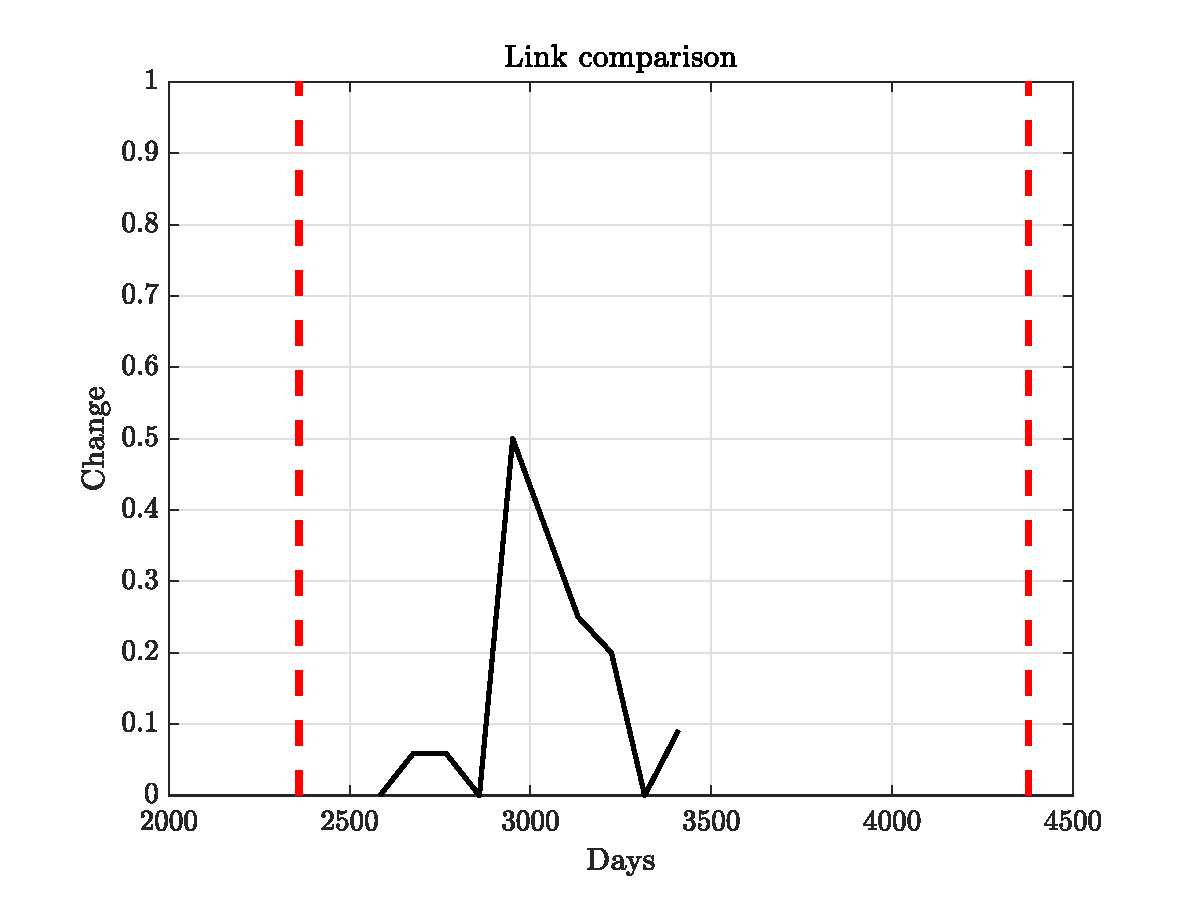
\includegraphics[width = 0.8\textwidth]{link_comparison}
    \caption{Red lines where new NDP leader selected.}
  \end{figure}
\end{frame}

\begin{frame}{Text comparison results}
  \begin{figure}
    \centering
    \includegraphics[width = 0.8\textwidth]{text_comparison}
    \caption{Red lines where new NDP leader selected.}
  \end{figure}
\end{frame}

\begin{frame}{Conclusions}
\begin{figure}
\centering     %%% not \center
\subfigure[Image comparison]{\label{fig:a}\includegraphics[width=52mm]{image_comparison}}
\subfigure[Text comparison]{\label{fig:b}\includegraphics[width=52mm]{text_comparison}}
\caption{Locations of high change correspond to new NDP leader selected.}
\end{figure}
\end{frame}

\begin{frame}{Conclusions}
\begin{itemize}
\item Different metrics are useful for different websites or for different types of change,
\begin{itemize}
\item e.g. news websites update content every day but this might not indicate significant change -- structural metric more informative than text metric,
\item e.g. governmental websites depend sensitively on text and content -- text metric most informative,
\item e.g. job registers will link to new advertisements -- link data most informative.
\end{itemize}
\vspace{2ex}
\item We see that the text, link and thumbnail metrics align for certain substantial changes.
\end{itemize}
\end{frame}

\end{document}